\documentclass[12pt]{article}
\usepackage{setspace, indentfirst, graphicx, enumitem}
\usepackage[vmargin=3.18cm,hmargin=2.54cm]{geometry}
\usepackage{fontspec}   %加這個就可以設定字體
\usepackage{xeCJK}       %讓中英文字體分開設置
\setCJKmainfont{AR PL UMing TW} %設定中文為系統上的字型,而英文不去更動,使用原TeX字型
\XeTeXlinebreaklocale "zh"             %這兩行一定要加,中文才能自動換行
\XeTeXlinebreakskip = 0pt plus 1pt     %這兩行一定要加,中文才能自動換行
\title{Design Pattern Final Project\\-- Social Network Search Engine}
\author{R00922009 楊詠翔, D98921028 王祐邦}

\begin{document}
\maketitle

\begin{figure}[t]
\centering
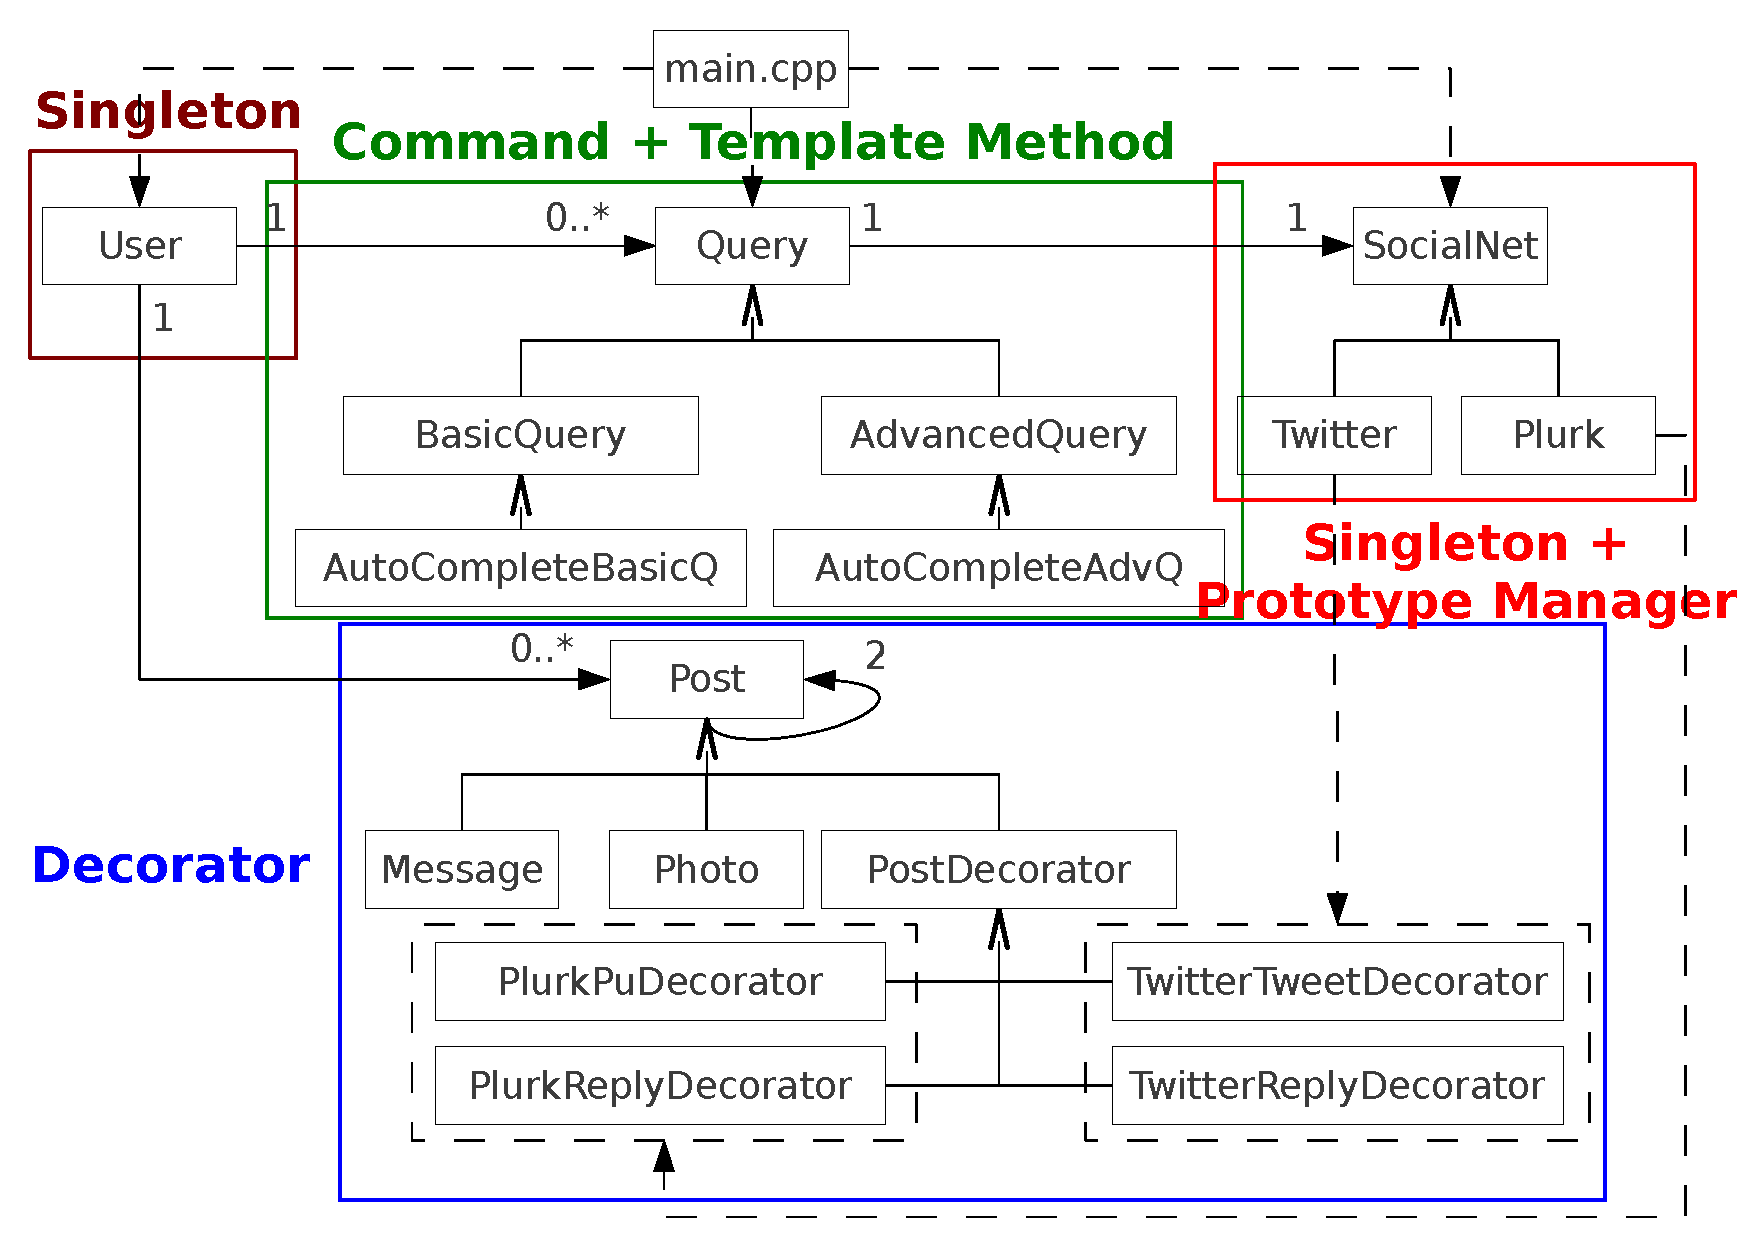
\includegraphics[width=15cm]{classDiagram+DP.pdf}
\caption{{\it The framework of our program}}
\label{fig:classDiagram}
\end{figure}

\section{簡介}

在本次期末專題中,我們這組以C++和Python實做了社群網站搜尋引擎,現階段支援Plurk以及Twitter的搜尋。主要的功能包括搜尋關鍵字和/或人名,瀏覽搜尋結果,還有推文以及回文的功能。

\section{系統架構與模式使用}

圖\ref{fig:classDiagram}是本組程式的系統架構(framework)。主要包括四個設計模式,將在接下來的段落說明。

\subsection{User -- Singleton}

首先,在program startup時,會instantiate一個User的instance,往後就只由這個User進行登入、登出、瀏覽等等。之所以在program startup就instantiate,是為了避免multi-thread問題。

\begin{figure}[t]
\centering
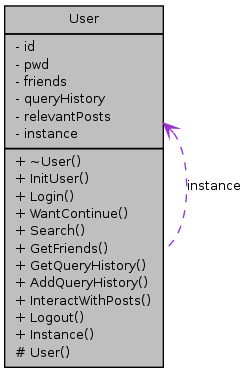
\includegraphics[width=5cm]{classUser__coll__graph.png}
\caption{{\it The collaboration graph of class User}}
\label{fig:classDiagram}
\end{figure}

\subsection{SocialNet -- Singleton + Prototype Manager}

我們想將social network也設計成Singleton,讓每次只有一個User跟一個SocialNet互動。然而由於SocialNet本身是Abstract Base Class,無法instance,同時也為了在不同的社群網站之間切換,我們將Prototype Manager跟Singleton結合在一起。

首先,在program startup時,每個SocialNet的derived class (Plurk, Twitter etc.)各自instantiate各自的Singleton (在圖\ref{fig:SocialNet_inherit}的private mambers "dummy"),並向SocialNet的Prototype Manager註冊。爾後當client code (main.cpp)想取得SocialNet的instance時,呼叫SocialNet::Instance(),SocialNet先將使用者要求的singleton of derived class複製(Clone)成自己的singleton,再回傳給User。如此一來也達到了避免multi-thread problem的功能,因為SocialNet::Instance()沒有New,只有Clone。

\begin{figure}[t]
\centering
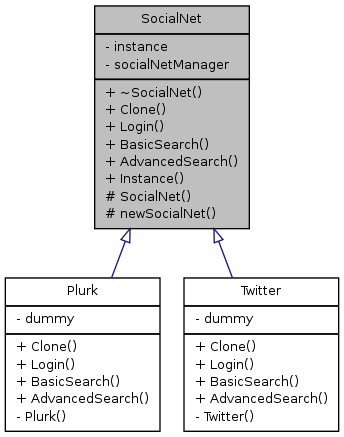
\includegraphics[width=7cm]{classSocialNet__inherit__graph.png}
\caption{{\it The inheritance graph of class SocialNet}}
\label{fig:SocialNet_inherit}
\end{figure}

\subsection{Query -- Command + Template Method}

圖\ref{fig:command}說明Query身為Command pattern與其他class的對應關係,同時也可用來說明我們系統的執行流程。首先由User透過Query::InitQuery()指定想要搜尋之關鍵字以及人名,之後Query再透過SocialNet的BasicSearch()或者AdvancedSearch(),經由Python腳本呼叫社群網站的API,進行相對應的搜索。最後再把搜尋結果return給User。

我們認為將Query實做成Command pattern是相當直覺的。第一是因為Query是由User指定,但是是由SocialNet執行。好比點菜的要求由服務生記錄,但是是由廚師執行一樣。第二是為了可以將Query歷史儲存起來,以便之後進行的自動完成功能。

\begin{figure}[t]
\centering
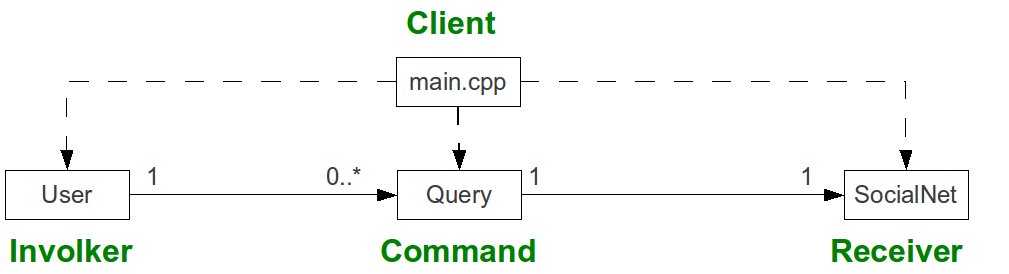
\includegraphics[width=15cm]{command.png}
\caption{{\it The collaboration graph of class Query}}
\label{fig:command}
\end{figure}

除了Command pattern以外,Query同時含有Template Method pattern。在圖\ref{fig:Query_inherit}中,class AutoCompleteBasicQ跟AutoCompleteAdvQ分別是為了override class BasicQuery跟AdvancedQuery所增加的derived classes。原本在BasicQuery跟AdvancedQuery,系統直接用cin要求使用者輸入關鍵字以及人名;而在AutoCompleteBasicQ跟AutoCompleteAdvQ,則是實現了自動完成的功能,稍候將在\ref{sec:autocomplete}節說明。

\begin{figure}[t]
\centering
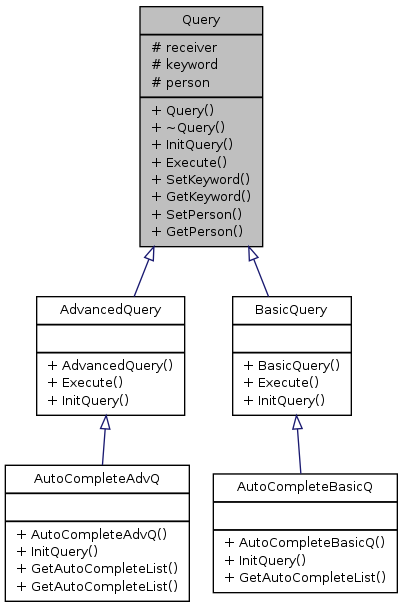
\includegraphics[width=7cm]{classQuery__inherit__graph.png}
\caption{{\it The inheritance graph of class Query}}
\label{fig:Query_inherit}
\end{figure}

\subsection{Post -- Decorator}

在尚未加上PostDecorator之前,class Post的主要methods包括印出自己的內容(Post::PrintContent()),還有提供前往上一篇、下一篇、或者結束瀏覽的選項(Post::PrintOption(),Post::ExecuteOption())。注意我們目前實做的concrete Post只有Message,而Photo當初雖然制定了介面,但沒有被使用過,只是為了示範其延伸性所以保留著。

而PostDecorator的目的,是為Post加上推文以及回文的功能。Concrete SocialNet在完成搜尋之後,負責create Post物件,並加上相對應的PostDecorator。每個concrete SocialNet對應到固定一組PostDecorator。因此換個角度講,SocialNet也可以視為Abstract Factory pattern,負責創造Post,並回傳給Query。

\begin{figure}[t]
\centering
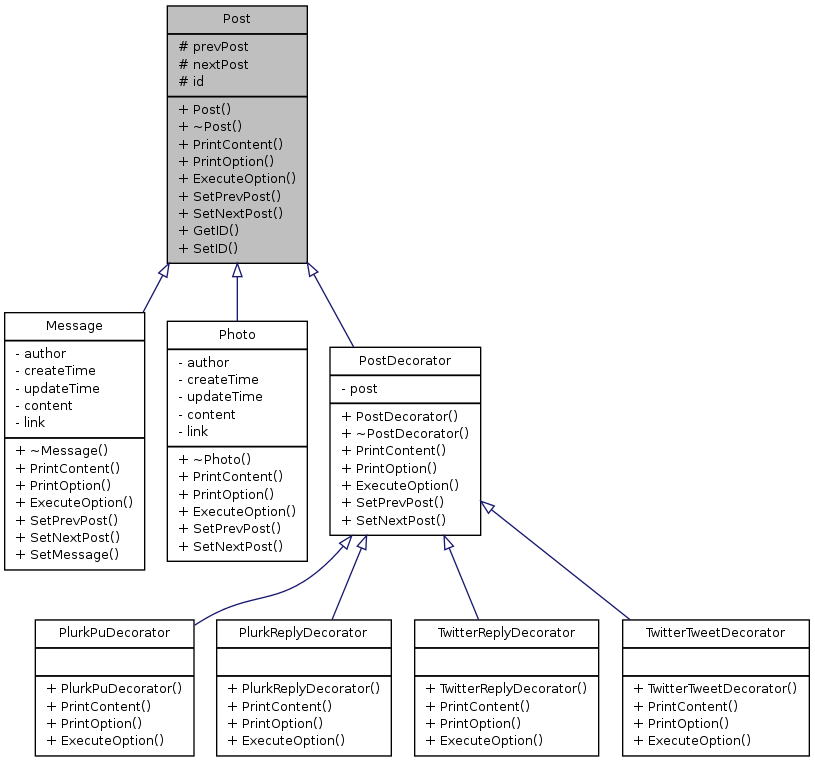
\includegraphics[width=15cm]{classPost__inherit__graph.png}
\caption{{\it The inheritance graph of class Post}}
\label{fig:Post_inherit}
\end{figure}

\section{社群網站API}

我們在實作社群網站搜尋系統的過程中使用了大量的API。由於各大社群網站的資料的存取方法以及傳遞規範不盡相同,即使大同小異,在實作上仍然有許多繁瑣的規定以及要求。所幸每個社群網站都有提供他本身的API原始碼操作說明,此外還有許多第三方的開放原始碼供所有欲開發者使用。我們這次總共實作了Plurk以及Twitter這兩個社群網站的搜尋,使用的API Library為  plurk-oauth by clsung 以及 tweepy by  joshthecoder : 這兩個都是Python Library for API,我們利用Library提供的函式實作了各種我們自定的功能,並且利用系統主程式(c++)呼叫額外寫的這部份的程式(python code)。

plurk api : http://www.plurk.com/API

twitter api : https://dev.twitter.com/docs/api

\subsection{Login}

由於目前大部分的social network api都是基於OAuth2的認證方式,所以為了讓不同使用者可以自由登入我們系統,我們找了OAuth2的python library來幫助我們完成登入的機制。我們讓初次使用的用戶在登入的時候指定到認證網頁輸入出正確的數字,就可以讓程式獲得所需要的Access Token,之後程式就可以利用該Access Token進行各種API的操作,而獲得的Access Token也會自動存下來,讓該使用者下一次登入的時候不需要再去索取Access Token。

\begin{figure}[t]
\centering
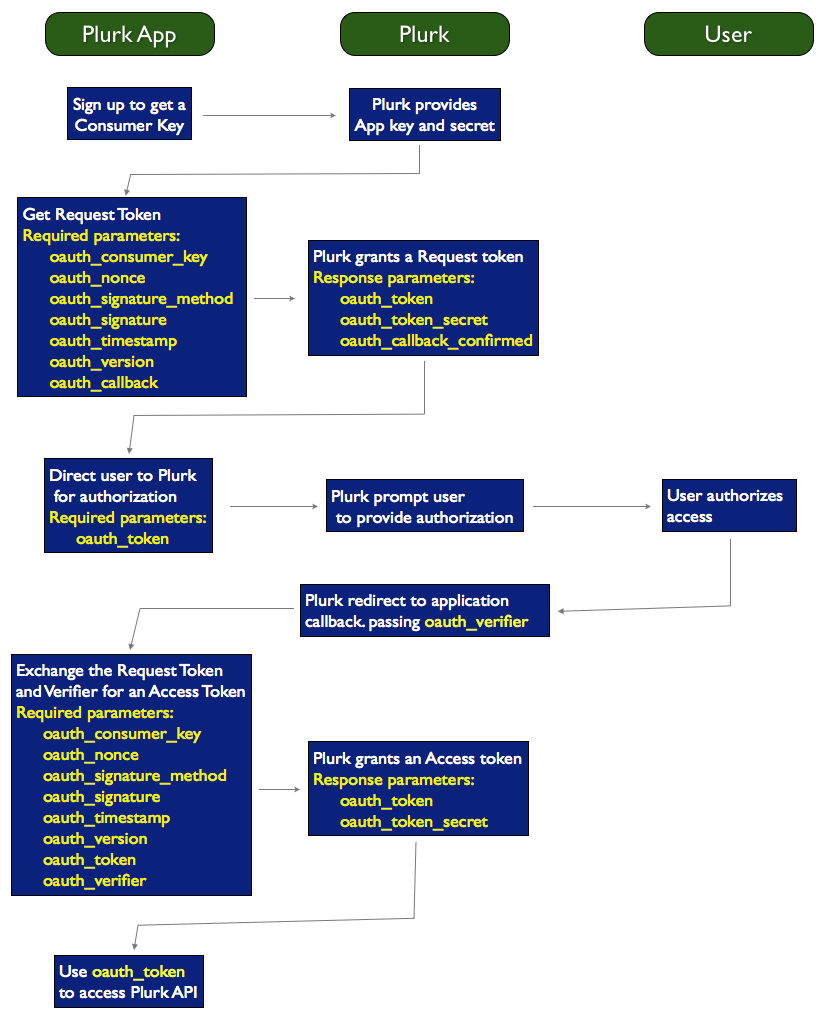
\includegraphics[width=15cm]{Plurk_Oauth.png}
\caption{{\it Plurk利用OAuth認證的流程圖,其他各大社群網站的方法亦同。}}
\label{fig:plurk_oauth}
\end{figure}

\subsection{Reply and Like}

這部份都是利用不同社群網站所提供的API來實作,我們只需要給定正確格式的參數,就可以實作搜尋,回覆,或是按讚等不同的功能。由於多數社群網站的回傳格式都是JSON格式,我們將其整理過後把我們程式需要的資料留下來存成檔案供我們的主程式去讀檔案。在系統中我們實作了兩種搜尋的方法,第一種是給定一個搜尋的關鍵字,對所有該社群網站的用戶所發的文章進行搜尋。這種方法是使用社群網站提供的API直接進行搜尋。 缺點是他不能過濾發文作者是否為用戶認識的人。所以我們額外實作了另外一種搜尋方法,其一是指定發文者以及關鍵字,我們先去取得所有該發文者所發的文章,再一一比對是否其文章中有出現關鍵字。另外一種是搜尋使用者的時間軸(在 Plurk 以及 Twitter 之中皆有 Timeline 的觀念)所有的文章,並且一一比對是否有關鍵字的出現。利用這種方法可以讓使用者找到身邊的朋友或是指定使用者的文章。

\section{其他特殊功能}
\label{sec:autocomplete}

除了搜尋、瀏覽、推文以及回文之外,我們還另外加了兩個功能。一個是Password Masking,也就是在輸入密碼的時候輸出"*"記號。另一個是自動完成。在搜尋時,輸入關鍵字以及人名的時候,按Tab即可自動完成。關鍵字是藉由搜尋使用者的過往的紀錄,系統會保留最近100次以內的關鍵字搜尋,在程式終止時寫成log檔,並在下次程式啟動時讀入。而人名則是搜尋好友名單。

\section{系統延伸性與未來展望}

本系統的設計足以提供包括新增社群網站(class socialNet)、文章類別(class Post)、與文章的互動方式(class PostDecorator)以及搜尋類別(class Query)。要新增社群網站,除增加socialNet的derived class,也要同時增加PostDecorator,以支援其推文、回文功能等等。同樣地,要增加文章類別或者與文章的互動方式,除增加Post、PostDecorator的derived class之外,也要修改或者新增socialNet。而如果要增加搜尋類別,除增加Query之外,也要修改或者新增socialNet,支援與該Query相對應的搜尋演算法。

而如果將來想要重構(refactor)程式碼,一個可能的方向是將Query::InitQuery()以及SocialNet::BasicSearch()、SocialNet::AdvancedSearch()以Bridge Pattern抽離出來。因為這些methods關聯緊密且可能時常需要擴充。

\section{編譯與執行}

本程式在Linux跟MacOS上測試過,介面為command line。直接在資料夾下執行make即可以g++編譯,並產生一名為bin的執行檔。

\section{分工}

R00922009 楊詠翔:負責社群網站API,並參與架構設計。

D98921028 王祐邦:負責系統架構設計、實做,以及增加特殊功能。

\end{document}
